\chapter{Background}

%---
\section{Data sources}
%---

% https://www.talend.com/resources/data-source/
% https://www.techopedia.com/definition/30323/data-source

A data source is what its name suggests, a location where the data that is being used originates from. A data source can be for example a database or a dynamic stream of data service such as constantly collecting the measured temperature in a room. In the context of this thesis project, we focus on database-like data sources, because in general, a visualization tool needs to be able to read the data to be displayed from a backend storage. \cite{talend-datasource} \cite{techopedia-datasource}

Concerning the types of databases, there are different categories, each with varying features and purposes. In the following sections, I briefly introduce some of the most used types of databases.

%---
\section{Relational database}
%---

% https://www.oracle.com/database/what-is-a-relational-database/
Probably the most popular type of databases is the relational database. It stores data points that are related to one another. Relational databases are based on a relational model, representing the data in tables. They are widely utilized in cases, when related data points need to be stored and managed in a secure, rules-based, consistent way. \cite{relational-database-oracle}

%---
\section{Time series database}
%---

%https://www.influxdata.com/time-series-database/

A time series database is optimized for storing time-stamped or time series data. Time series data are measurements that are tracked and aggregated over time. This could be metrics about servers, application performance, network data, etc. A time series database possesses enhanced capabilities to handle the measurement of change over time compared to other types of databases. \cite{timeseries-database-influxdata}

%---
\section{Key-Value database}
%---

% https://aws.amazon.com/nosql/key-value/

A key-value database is type of nonrelational database that uses a simple key-value method to store data. The data is stored as a collection of key-value pairs in which the key fulfills the role of a unique identifier. Both the keys and the values can have any type, simple objects, like number or string or even complex compound objects. This means that the schema of the data is defined per item, instead of on a collection or table level, like in the case of relational databases. Key-value databases are mostly utilized for cache management or storing information in session-oriented applications. \cite{keyvalue-database-aws}

%---
\section{Document database}
%---

% https://aws.amazon.com/nosql/document/

Document databases are another type of nonrelational database that is designed to store and query the recorded information as flexible, semistructured JSON-like documents. They make it easier for developers to handle data in the database by using the same document-model format they use in their application code. Document databases allow flexible indexing and powerful ad hoc queries. \cite{document-database-aws}

%\begin{itemize}
%	\item data sources and their features, use-cases, pros/cons?
%	\begin{itemize}
%		\item relational db
%		\item timeseries
%		\item key-value
%		\item document
%	\end{itemize}
%	\item with examples!
%\end{itemize}


%--
\section{Grafana}
%--

% from grafana.com
Grafana is one of the most popular open source analytics and monitoring solution that can be connected to the majority of the main data sources out-of-the-box. It allows its users to query, visualize and alert on the collected metrics. 

Altough Grafana has got plenty of useful feature, only those relevant to the scope of the thesis project will be briefly explained here

%--

%---
%https://grafana.com/docs/guides/basic_concepts/#data-source
\subsection{Data Source}

Grafana supports many different storage backends (Data Source). Each Data Source has a specific Query Editor (see later in section \ref*{query-editor}) that is customized for the features and capabilities that the particular Data Source exposes. Of course, this leads to the fact that the query language and capacity of each Data Source are obviously very different. \cite{grafana-datasource}

Grafana mainly favors time series data (e.g. from Prometheus or InfluxDB), but it can work with other types of data source (e.g. relational databases (MySQL, PostgreSQL, MSSQL), logging and document databases (Loki, Elasticsearch)).

% https://grafana.com/docs/guides/basic_concepts/#panel
\subsection{Panel}

The Panel is the basic visualization building block in Grafana. Each Panel provides a so called Query Editor (dependent on the Data Source selected in the panel) that allows the user to create data source specific queries (e.g. an SQL query for a MySQL data source) in order to extract the desired metrics as precisely as possible. \cite{grafana-panel}

There are multiple built-in Panel types available in Grafana, however, custom panels made by the open source community are also accessible. Probably the most widely used Panel types are the Graph, Table, Singlestat and Gauge. An example of the Graph Panel can be viewed in Figure \ref{fig:graph-panel}.

\begin{figure}[h]
	\centering
	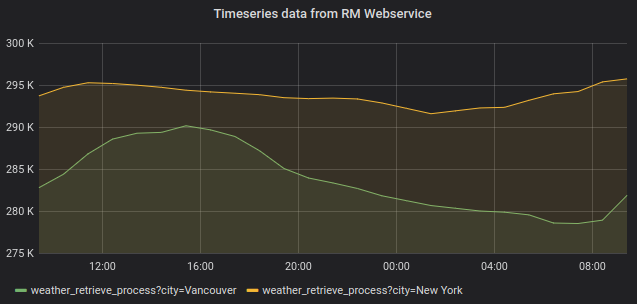
\includegraphics[width=130mm, keepaspectratio]{figures/graph-panel-medium.png}
	\caption{Graph Panel}
	\label{fig:graph-panel}
\end{figure}

%https://grafana.com/docs/grafana/latest/guides/basic_concepts/#query-editor
\subsection{Query Editor}\label{query-editor}

The Query Editor exposes the capabilities of the Data Source and allows the user to query the metrics that it contains. The queries created in the Query Editor of a panel determine what data will be displayed on the panel. \cite{grafana-queryeditor} An example Query Editor is shown in Figure \ref{fig:query-editor}.

\begin{figure}[H]
	\centering
	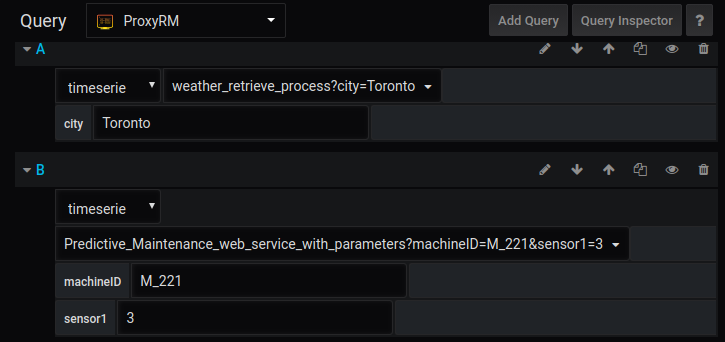
\includegraphics[width=130mm, keepaspectratio]{figures/query-editor.png}
	\caption{Query Editor}
	\label{fig:query-editor}
\end{figure}

%---
\subsection{Dashboard}
%---
% https://grafana.com/docs/grafana/latest/guides/basic_concepts/#dashboard
The Dashboard is where all the previously mentioned building blocks come together. Dashboards can be thought of as an organized set of Panels. \cite{grafana-dashboard}

We can use the Dashboard to visualize different metrics in one, easily manageable place. This is quite useful, when many aspects must be taken into account in order to be able to thoroughly understand our currently inspected data set. An example Dashboard about a Kubernetes cluster can be viewed in Figure \ref{fig:dashboard}.

%\begin{center}
%	--- TODO insert reference for img
%	% https://grafana.com/grafana/dashboards/8670
%\end{center}

\begin{figure}[H]
	\centering
	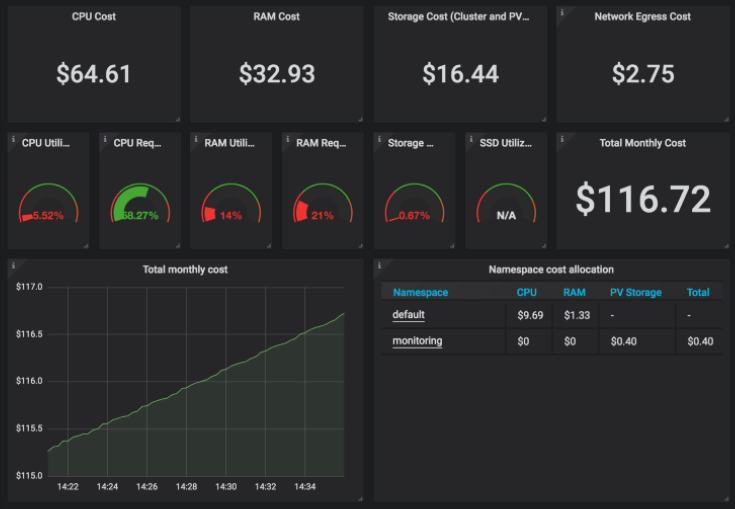
\includegraphics[width=130mm, keepaspectratio]{figures/dashboard-small.png}
	\caption{Dashboard https://grafana.com/grafana/dashboards/8670}
	\label{fig:dashboard}
\end{figure}

%---
\subsection{Interactivity in general}
%---
When working with and visualizing massive amount of data is a major part of one's profession, it can be quite convenient if the tools can provide the ability to allow some user-interaction. Meaning that the user do not have to work with static diagrams or rewrite complex configurations so that he or she is capable of further analyzing the collected data.

% retelabor2 vizualis adatelemzes (http://docs.inf.mit.bme.hu/remo-jegyzet/vizualis-adatelemzes-konyvfejezet.pdf)
Commonly available interactivity options can be the followings \cite{visual-analysis}:
\begin{itemize}
	\item \emph{statistic indicators} - easily accessible statistic information (e.g. average value, spread-diagram) about individual objects shown on the diagram (this is usually achieved by mouse-hovering)
	\item \emph{local interactions} - changing the outlook of a diagram without affecting other displayed objects (e.g. reordering the bars on a bar-chart, rescaling the axis on a graph or other diagram-specific modifications)
	\item \emph{selection and linked highlighting} - when we have multiple diagrams displaying different views of the same data set, selecting a subset of the data on one diagram (e.g. a bar on a bar-chart) highlights that particular part of the data on another diagrama (e.g. a set of points on a scatter-plot)
	\item \emph{linked analysis}- for example, selecting a subset of the data triggers a reactive analysis, creating a statistic model (regression, scatter-plot, spread-diagram) using that specific data set
\end{itemize}

%---
\subsection{Interactivity in Grafana}
%---

While it is hard to find a tool, which possesses all the before-mentioned interactivity capabilities, Grafana provides certain features to enable efficient user-interaction for the good of solid understanding of the data.


% https://grafana.com/docs/reference/timerange/
%---
\subsubsection{Time Range Controls}
%---

Grafana provides numerous ways to interactively manage the time ranges of the data being visualized. \cite{grafana-time-range-controls}

On the Dashboard-level, the 'Current time range' selector can be used to change the dashboard time. Doing this refreshes the whole dashboard with each panel on it. Those panels, which display time-dependent information, will only show data-points which timestamps are in the newly set time range.

If there is a Graph Panel on the dashboard, there is another possibility to change the Dashboard-level time range. We can select a time range on the Graph Panel with the cursor. This method is quite effective in case, when we would like to swiftly zoom into our data to review more refined details. An example for that feature is displayed in Figure \ref{fig:select-time}.

\begin{figure}[h]
	\centering
	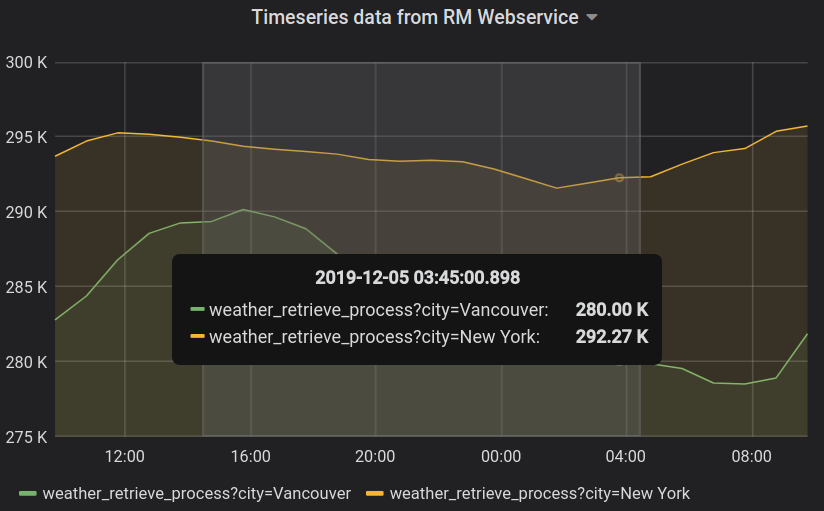
\includegraphics[width=130mm, keepaspectratio]{figures/select-time.png}
	\caption{Zoom into the time range}
	\label{fig:select-time}
\end{figure}

% https://grafana.com/docs/reference/templating/
%---
\subsubsection{Variables and Templating}
%---

Variables in Grafana allow for more interactive and dynamic dashboards. We can use variables in metric queries and in panel titles.

Their role is similar to that of 'conventional' variables in programming languages. Instead of hard-coding things into the program, we can use them to create algorithms, that operate on a more abstract level, resulting in more effortlessly maintainable softwares.

In Grafana, we can use the variables to write generalized metric queries. For example, if we have multiple servers and we have metric data from all of them, we could store the name or address of the servers in a variable, rather than defining numerous queries, which only differ in the server name. Variables are shown as dropdown select boxes at the top of the dashboard. These dropdowns make it easy to change the value of each available variable, thus to adjust the data being displayed in the dashboard.\cite{grafana-variables} An example of that can bee seen in Figure \ref{fig:variable-dropdown}.

\begin{figure}[H]
	\centering
	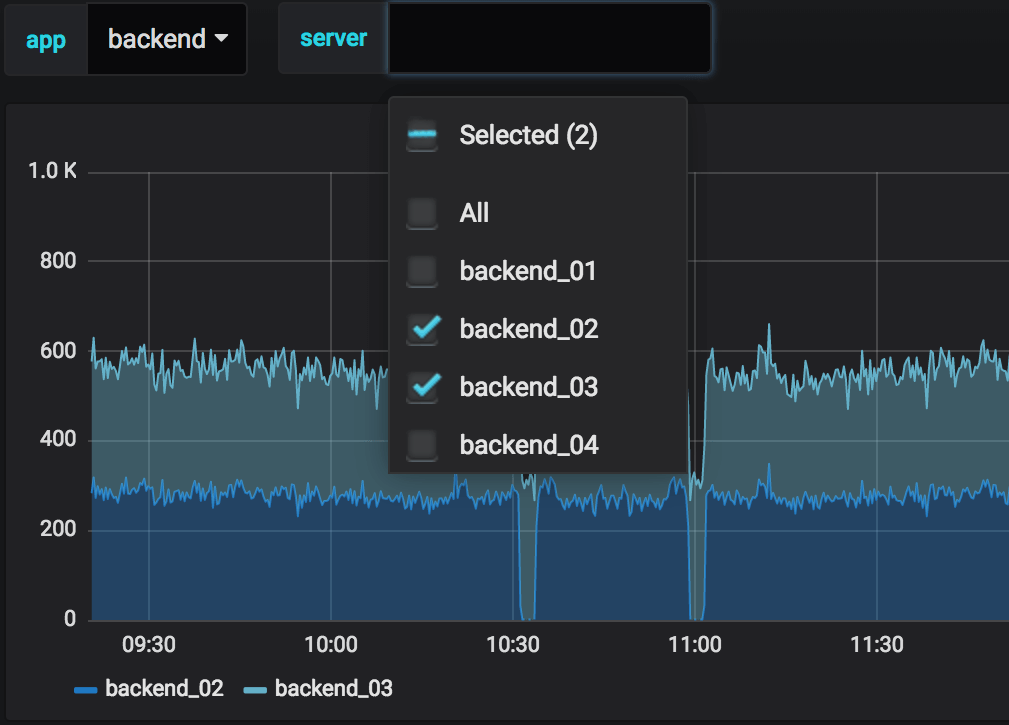
\includegraphics[width=130mm, keepaspectratio]{figures/variable-dropdown.png}
	\caption{Variable dropdown \cite{grafana-variables-dashboard-image}}
	\label{fig:variable-dropdown}
\end{figure}

% https://grafana.com/static/img/docs/v50/variables_dashboard.png

% https://grafana.com/docs/reference/templating/#variable-types
There are different types of variable that can be used to make dashboards more dynamic.\cite{grafana-variables-types}
\begin{itemize}
	\item \emph{Query} - This variable type allows for writing a data source query that usually returns a list of metric names. For example, a query that returns a list of server names, sensor ids, or data centers.
	\item \emph{Interval} - This variable can represent time spans. We can use them, when we need to aggregate data-points by time or date.
	\item \emph{Data source} - This type makes it possible to quickly change the data source for an entire Dashboard. This feature can be quite suitable, when we have multiple instances of a data source in for example different environments.
	\item \emph{Custom} - This variable can be used to manually define the value options for the given variable.
	\item \emph{Constant} - This variable can be handy for example to easily declare metric path prefixes. 
	\item \emph{Text box} - This variable type displays as a free text input field with an optional default value.
	\item \emph{Ad hoc filters} - It is a quite special kind of variable that only works with some data sources (e.g. InfluxDB, Elasticsearch). It allows the user to add key/value filters that will automatically be added to all metric queries the use the specified data source.
\end{itemize}

%---
\subsubsection{Basic statistic values in legend}
%---

Statistic indicators were already mentioned above, where we discussed interactivity in general. In Grafana, we can display some basic statistic values (minimum, maximum, average, total) in the Graph Panel. An illustration of this feature is displayed in Figure \ref{fig:basic-statistics}.

\begin{figure}[H]
	\centering
	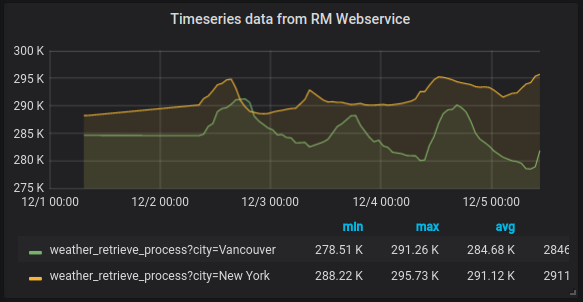
\includegraphics[width=130mm, keepaspectratio]{figures/basic-statistics.png}
	\caption{Basic statistic values on Graph Panel}
	\label{fig:basic-statistics}
\end{figure}

% https://grafana.com/docs/features/panels/graph/#data-link
%---
\subsubsection{Data links}
%---

Data links provide a way to add dynamic links to the visualization. These links can link to either other dashboards or to an external URL. When using data links, additional built-in variables become available that enable creating dynamic links.\cite{grafana-graph-datalink}

These variables are:
\begin{itemize}
	\item \emph{\char`_\char`_series\char`_name} - the name of the series or the table
	\item \emph{\char`_\char`_value\char`_time} - the timestamp of the point that is clicked on (in millisecond epoch)
	\item \emph{\char`_\char`_url\char`_time\char`_range} - The current time range
	\item \emph{\char`_\char`_all\char`_variables} - Adds all current variables and their current values to the URL
\end{itemize}

%---
\subsubsection{Creating custom interactivity}
%---

As Grafana is a fully open source project, it is possible for the community, to develop custom objects in Grafana or to extend built-in ones. This way, it is achievable to create custom interactivity features according to the needs of the user.


%\begin{itemize}
%	\item what is Grafana?
%	\begin{itemize}
%		\item dashboard
%		\item panel
%		\item datasource
%		\item queries
%		\item query editor (because of extended ui - dynamic parameter listing))
%	\end{itemize}
%	\item connects with many main datasources
%	\item customizable, can write own plugins (panel, datasource, app)
%	\item interactivity features
%	\begin{itemize}
%		\item what can be meant as interactivity in this context (retelab2 lab segedlet)
%		\item variables, templating
%		\item setting the time-range
%		\item customizing builtin Graph Panel
%		\item data-links in Graph Panel
%		\item panel links (formerly drill-down links)?
%	\end{itemize}
%\end{itemize}

%---
\section{RapidMiner}
%---

% https://rapidminer.com/us/
% https://en.wikipedia.org/wiki/RapidMiner
% https://docs.rapidminer.com/latest/server/overview/scalable-architecture.html

RapidMiner is a data science software platform that provides an integrated environment for data preparation, machine learning, deep learning, text mining and predictive analytics.

RapidMiner includes several components, however, only the ones with relevant features to this thesis project are introduced briefly in this section.

%---
\subsection{RapidMiner Server}
%--- 

RapidMiner Server is the central component in the architecture. Users can interact with it via a web interface or via RapidMiner Studio.

Its main responsibilities are to store and expose data science processes, like model building, predictions, data ETL (Extract, Transform, Load) operations, etc. Long-running jobs are executed externally via Job Agents. The RapidMiner Server stores its data in an external database.

%---
\subsubsection{Web services}
%---
The Server can expose certain processes that can be invoked via simple HTTP requests. These are the so called web services which can be used to run predictions or any other application of models, where the need for a real-time response is paramount. In order to make this service more dynamic, additional parameters can be sent with the requests to get more accurate information. The user can acquire the results of these processes through the same API in JSON format.

%---
\subsection{Job Agent}
%---

RapidMiner Server offers a queue system for long-running jobs, which are executed externally via Job Agents. The computing power of the stack can be increased by adding more Job Agents.

%--
\section{JSON}
%--

% https://www.json.org/json-en.html
% https://www.w3schools.com/whatis/whatis_json.asp

In this thesis project, I use the JSON data-interchange format to send information between the various components. For this reason, a brief description of the JSON format is appropriate in this chapter.

The JSON stands for Javascript Object Notation and it is a lightweight format for storing and transporting data. We can say that JSON is easily read by both humans and machines, as a JSON object is merely an unordered set of name/value pairs. The name is a string and the values can be different types of data, for example a number, a string, an array or another object. These types are supported in all modern programming languages in one form or another, thus despite what its name suggest, the JSON format can be regarded as an universal data structure. An example JSON object can be seen in the code snippet Listing \ref{lst:json-example}.

\begin{center}
	\begin{minipage}{0.6\linewidth}
		\begin{lstlisting}[language=Python, caption={Example JSON}, label={lst:json-example}]]
		{
		  "name": "Test",
		  "age": 23,
		  "car": {
		    "type": "van"
		  },
		  "languages": ["english", "french"]
		}
		\end{lstlisting}
	\end{minipage}
\end{center}





